\documentclass[conference]{IEEEtran}
\usepackage[utf8]{inputenc}
\usepackage[T1]{fontenc}
\usepackage[turkish]{babel}
\usepackage{amsmath,amssymb,amsfonts}
\usepackage{algorithmic}
\usepackage{algorithm}
\usepackage{graphicx}
\usepackage{textcomp}
\usepackage{xcolor}
\usepackage{booktabs}
\usepackage{stfloats}
\usepackage{cite}

\addto\captionsturkish{
  \renewcommand{\figurename}{Şekil}
  \renewcommand{\tablename}{Çizelge}
  \renewcommand{\abstractname}{Özet}
  \renewcommand{\IEEEkeywordsname}{Anahtar Kelimeler}
  \renewcommand{\refname}{KAYNAKLAR}
}

\let\scshape\upshape
\renewcommand{\IEEEiedlistdecl}{\setlength{\itemsep}{1pt}\setlength{\parskip}{0pt}\setlength{\topsep}{2pt}}

\floatname{algorithm}{Algoritma}
\renewcommand{\algorithmicrequire}{\textbf{Girdi:}}
\renewcommand{\algorithmicensure}{\textbf{Çıktı:}}

\renewcommand{\topfraction}{0.95}
\renewcommand{\bottomfraction}{0.85}
\renewcommand{\textfraction}{0.05}
\renewcommand{\floatpagefraction}{0.75}
\renewcommand{\dbltopfraction}{0.95}
\renewcommand{\dblfloatpagefraction}{0.75}

\begin{document}
\shorthandoff{=}

\title{Kampüs Kaynak Rezervasyon Sistemi}

\author{\IEEEauthorblockN{Yiğit Karabacak}
\IEEEauthorblockA{\textit{Bilgisayar Mühendisliği Bölümü} \\
\textit{Kocaeli Üniversitesi}\\
Kocaeli, Türkiye \\
240201025@kocaeli.edu.tr}
}

\maketitle

\begin{abstract}
Ortak kullanıma açık kurumsal ve akademik kaynakların (toplantı odaları, laboratuvarlar, 3D yazıcılar ve GPU sunucuları) eşzamanlı paylaşımı; zaman çakışmaları, hazırlık ve bakım süreleri, bakiye kotaları ve kullanıcı güvenilirliği gibi kısıtların birlikte yönetilmesini gerektirir. Bu çalışmada, Kocaeli Üniversitesi Yazılım Laboratuvarı~I kapsamında, kampüs içi kaynak tahsisini yöneten kural tabanlı bir rezervasyon modülü ile bu modülü doğrudan kullanan bir masaüstü uygulaması geliştirilmiştir. Sistem, harici paket gerektirmeden Python 3.11 standart kütüphanesi üzerinde dört katmanlı (modeller, dinamik ücretlendirme, çekirdek durum makinesi ve kullanıcı arayüzü) olarak tasarlanmıştır. Ücretlendirme, 15 dakikalık dilimler ve iki saatlik yedi bant üzerinden doluluk oranı ve pik saat çarpanlarıyla hesaplanan Kaynak Puanı (KP) ekonomisine dayanır. Rezervasyon talepleri 13 adımlı doğrulama sırasından geçirilir; çakışma durumunda güvenilirlik puanına göre sıralanan bekleme listesi işletilir ve simüle saat ilerletildiğinde aradaki olaylar kronolojik sırayla yürütülür. Geliştirilen sistem, şartnamenin 19 komutluk referans senaryosunda ve sınır değerleri sınayan 72 komutluk test kümesinde beklenen sonuçlarla alan ve tip düzeyinde birebir eşleşmiştir.
\end{abstract}

\begin{IEEEkeywords}
Kaynak rezervasyonu, durum makinesi, dinamik ücretlendirme, olay güdümlü simülasyon, bekleme listesi, yazılım mimarisi, Tkinter GUI.
\end{IEEEkeywords}

\section{GİRİŞ}
Üniversite yerleşkelerinde sınırlı sayıdaki teknik donanımın ve çalışma alanlarının araştırmacılar, teknisyenler ve öğrenciler arasında paylaşımı, basit takvim çakışma kontrolünün ötesinde kurallar gerektirir. Cihazların iki kullanım arasındaki hazırlık gereksinimleri (üç boyutlu yazıcıların soğuma süresi, laboratuvarların havalandırılması), enerji tüketim profilleri, planlı bakım pencereleri ve kullanıcıların rezervasyonlarına uyma oranları kaynak kullanımını doğrudan etkiler~\cite{coffman1996, rexford2009}.

Bu çalışmada, aşağıdaki gereksinimleri karşılayan modüler bir rezervasyon sistemi geliştirilmiştir:
\begin{enumerate}
    \item \textbf{Kaynak Puanı (KP) Ekonomisi:} Talep yığılmasını önlemek için kullanıcılara rollerine göre haftalık KP kotası verilir ve bakiyeler her Pazartesi 00:00'da yenilenir.
    \item \textbf{Dinamik Fiyatlandırma:} Günün saatine (10:00--16:00 pik saatleri) ve ilgili kaynak türünün iki saatlik banttaki doluluk oranına göre 15 dakikalık dilimler üzerinden ücret hesaplanır.
    \item \textbf{Hazırlık ve Bakım Kısıtları:} İki kullanım arasında kaynak türüne özgü hazırlık süresi korunur ve bakım pencereleriyle kesişen talepler reddedilir.
    \item \textbf{Güvenilirlik Puanı:} Rezervasyonuna gelmeyen veya başlangıca 2 saatten az kala iptal eden kullanıcıların güvenilirlik puanı düşürülür; bu puan bekleme listesindeki sırayı ve ileri tarih sınırını belirler.
    \item \textbf{Katmanlı Mimari:} Çekirdek modül, komut satırından JSON Lines akışıyla çalışabilen bağımsız bir durum makinesi olarak yazılmış; masaüstü uygulaması ise iş kuralı barındırmadan doğrudan bu modülü çağıran bir arayüz katmanı olarak kurgulanmıştır.
\end{enumerate}

\section{YÖNTEM VE SİSTEM MİMARİSİ}
Sistem, sorumlulukların ayrılığı (\textit{Separation of Concerns}) ilkesi doğrultusunda birbirine gevşek bağlı dört temel modül halinde yapılandırılmıştır (Şekil~\ref{fig:mimari}).

\begin{figure}[H]
\vspace{-4pt}
\centering
\small
\setlength{\fboxsep}{3pt}
\fbox{
\begin{minipage}{0.94\columnwidth}
\centering
\textbf{KULLANICI ARABİRİMLERİ KATMANI}\\[1pt]
\fbox{\parbox{0.44\columnwidth}{\centering \scriptsize \textbf{Masaüstü Arayüzü (GUI)}\\\texttt{arayuz.py}}} \hfill
\fbox{\parbox{0.44\columnwidth}{\centering \scriptsize \textbf{Komut Satırı (CLI)}\\\texttt{main.py}}}
\\[2pt]
$\boldsymbol{\downarrow}$ \scriptsize \textit{JSON Formatında Komut / Doğrudan Çağrı} $\boldsymbol{\downarrow}$\\[1pt]
\textbf{ÇEKİRDEK REZERVASYON MOTORU (\texttt{motor.py})}\\[1pt]
\fbox{\parbox{0.44\columnwidth}{\centering \scriptsize K10 Doğrulama Hiyerarşisi}} \hfill
\fbox{\parbox{0.44\columnwidth}{\centering \scriptsize K8 Durum Geçiş Makinesi}}\\[1pt]
\fbox{\parbox{0.44\columnwidth}{\centering \scriptsize K7 Atomik Paket Denetimi}} \hfill
\fbox{\parbox{0.44\columnwidth}{\centering \scriptsize K9 Öncelikli Bekleme L.}}\\[1pt]
\fbox{\parbox{0.44\columnwidth}{\centering \scriptsize K11 Dinamik Olay Döngüsü}} \hfill
\fbox{\parbox{0.44\columnwidth}{\centering \scriptsize K3--K4 Hazırlık \& Ardışık}}
\\[2pt]
$\boldsymbol{\downarrow}$ \scriptsize \textit{Dinamik Ücret Hesabı \& Veri İşleme} $\boldsymbol{\downarrow}$\\[1pt]
\textbf{ALTYAPI VE VERİ KATMANI}\\[1pt]
\fbox{\parbox{0.44\columnwidth}{\centering \scriptsize \textbf{Dinamik Ücretlendirme}\\\texttt{ucretlendirme.py}}} \hfill
\fbox{\parbox{0.44\columnwidth}{\centering \scriptsize \textbf{Veri Modelleri}\\\texttt{modeller.py}}}
\end{minipage}
}
\vspace{-2pt}
\caption{Kampüs Kaynak Rezervasyon Sistemi Modüler Mimarisi.}
\label{fig:mimari}
\vspace{-4pt}
\end{figure}

\subsection{Veri Modeli ve Bellek İçi Yapılar}
Yapılandırma verileri çalışma anında \texttt{baslangic.json} dosyasından okunarak nesneleştirilir. Proje şartnamesi~\cite{yazlab2026} gereği veritabanı kullanılmamış; tüm durum bellekte (RAM) \texttt{@dataclass} yapılarıyla tutulmuştur (\texttt{YYYY-AA-GGTSS:DD}):
\begin{itemize}\raggedright
    \item \textbf{KaynakTuru:} \texttt{ad}, \texttt{hazirlik\_dk}, \texttt{temel\_ucret}, \texttt{enerji\_yogun}, \texttt{sertifika}.
    \item \textbf{Rol:} \texttt{ad}, \texttt{haftalik\_kota}, \texttt{ileri\_gun}, \texttt{azami\_sure\_dk}.
    \item \textbf{Kaynak:} \texttt{id}, \texttt{ad}, \texttt{tur}, \texttt{izinli\_roller}.
    \item \textbf{Kullanici:} \texttt{id}, \texttt{ad}, \texttt{rol}, \texttt{sertifikalar}, \texttt{bakiye}, \texttt{guvenilirlik} ($\in [0, 100]$).
    \item \textbf{Rezervasyon:} \texttt{id}, \texttt{kullanici}, \texttt{kaynak}, \texttt{baslangic}, \texttt{bitis}, \texttt{ucret}, \texttt{durum}, \texttt{paket}.
    \item \textbf{BakimPenceresi:} \texttt{kaynak}, \texttt{baslangic}, \texttt{bitis}.
    \item \textbf{BeklemeKaydi:} \texttt{id}, \texttt{kullanici}, \texttt{kaynak}, \texttt{baslangic}, \texttt{bitis}, \texttt{kayit\_saati}.
\end{itemize}

\subsection{Dinamik Ücretlendirme Motoru (K5)}
Rezervasyon ücretleri, kaynağın saatlik temel ücreti, talep edilen aralığın doluluk oranı ve günün zaman dilimi dikkate alınarak 15 dakikalık ayrık dilimler üzerinden hesaplanır:
\begin{equation}
\text{ücret} = \text{yuvarla}\left(\sum_{\text{dilim}} \text{temel\_ucret} \times 0{,}25 \times \text{bc} \times \text{pc}\right)
\label{eq:ucret}
\end{equation}
Burada $\text{bc}$ bant çarpanını, $\text{pc}$ ise pik çarpanını temsil eder:
\begin{enumerate}
    \item \textbf{Zaman Bantları:} Gün, 08:00--22:00 arasında ikişer saatlik yedi banda ayrılmıştır: $B \in \{08\text{--}10, \dots, 20\text{--}22\}$.
    \item \textbf{Doluluk Oranı:} İlgili bant ve kaynak türü için talep anındaki doluluk oranı şu şekilde bulunur:
    \begin{equation}
    \text{doluluk} = \frac{\text{banttaki toplam dolu dakika}}{\text{ilgili türdeki aktif kaynak sayısı} \times 120}
    \end{equation}
    Yalnızca \texttt{ONAYLI} ve \texttt{KULLANIMDA} rezervasyonlar sayılır; talebin kendisi ve bakım pencereleri sayılmaz. \texttt{kaynak\_ekle} ile eklenen kaynaklar paydaya katılır.
    \item \textbf{Bant Çarpanı:} Doluluk oranına göre 5 kademeli merdiven fonksiyonu işletilir ($1 + 0{,}25 \times \lfloor 4 \times \text{doluluk} \rfloor$):
\end{enumerate}

\begin{table}[H]
\vspace{-4pt}
\caption{DOLULUK ORANI VE BANT ÇARPANI KATSAYILARI}
\label{tab:doluluk}
\centering
\begin{tabular}{lc}
\toprule
\textbf{Doluluk Aralığı} & \textbf{Bant Çarpanı ($\text{bc}$)} \\
\midrule
$0{,}00 \le \text{doluluk} < 0{,}25$ & 1,00 \\
$0{,}25 \le \text{doluluk} < 0{,}50$ & 1,25 \\
$0{,}50 \le \text{doluluk} < 0{,}75$ & 1,50 \\
$0{,}75 \le \text{doluluk} < 1{,}00$ & 1,75 \\
$\text{doluluk} = 1{,}00$ & 2,00 \\
\bottomrule
\end{tabular}
\vspace{-4pt}
\end{table}

\begin{enumerate}
    \setcounter{enumi}{3}
    \item \textbf{Pik Çarpanı:} 10:00--16:00 arası pik saatlerdir. Tür \texttt{enerji\_yogun: true} ise pik dilimlerde $1{,}5$, aksi halde $1{,}0$'dır.
    \item \textbf{Yuvarlama:} Dilim ücretlerinin toplamı yarım-yukarı (\textit{round half-up}, $\ge 0{,}5$ yukarı) kuralıyla tam sayıya yuvarlanır (\texttt{math.floor(toplam + 0.5)}).
\end{enumerate}

\subsection{K10 Doğrulama Sırası ve Kural Hiyerarşisi}
Çekirdek motor, şartname K10'da tanımlı 13 aşamalı hiyerarşiyi sırasıyla yürütür ve ilk karşılaşılan ihlalin kodunu döner:
\begin{enumerate}
    \item \texttt{BULUNAMADI}: Kullanıcı veya kaynak ID'si tanımsız.
    \item \texttt{ZAMAN\_ADIMI\_HATASI}: 15 dk adımı dışı veya bitiş $\le$ başlangıç.
    \item \texttt{GECMIS\_ZAMAN}: Başlangıç saati $<$ mevcut simüle saat.
    \item \texttt{CALISMA\_SAATI\_DISI}: Gün aşımı veya 08:00--22:00 dışı.
    \item \texttt{SURE\_SINIRI}: Süre $<30$ dk veya rol azami süresinden fazla.
    \item \texttt{ILERI\_TARIH\_SINIRI}: İleri gün sınırı aşımı (Güvenilirlik $<50$ ise 1 gün).
    \item \texttt{ROL\_IZNI\_YOK}: Kullanıcı rolü kaynak izinli rollerinde yok.
    \item \texttt{SERTIFIKA\_YOK}: Türün gerektirdiği sertifika eksik.
    \item \texttt{BAKIM}: Bakım penceresiyle kesişme mevcut.
    \item \texttt{KESISME}: ONAYLI/KULLANIMDA rezervasyonla çakışma.
    \item \texttt{HAZIRLIK\_IHLALI}: Hazırlık süresi (\texttt{hazirlik\_dk}) boşluğu ihlali.
    \item \texttt{ARDISIK\_KULLANIM}: Aynı kullanıcı ve kaynakta $<60$ dk boşluk.
    \item \texttt{BAKIYE\_YETERSIZ}: Kullanıcının KP bakiyesi yetersiz.
\end{enumerate}

\subsection{Özel Kısıtlar ve Doğrulama Kuralları (K3, K4, K7, K9)}
\begin{itemize}
    \item \textbf{K3. Hazırlık Süresi Kısıtı:} Kaynağın iki kullanım arasında soğuması/havalandırılması için gereken süre $h$ (\texttt{hazirlik\_dk}) olmak üzere; yeni talep $[b, e)$ ile mevcut \texttt{ONAYLI}, \texttt{KULLANIMDA} veya \texttt{TAMAMLANDI} rezervasyon $[b', e')$ çakışmasa bile $b < e' + h \land e + h > b'$ ise \texttt{HAZIRLIK\_IHLALI} döner (\texttt{IPTAL} ve \texttt{GELMEDI} sayılmaz).
    \item \textbf{K4. Art Arda Kullanım Sınırı:} Aynı kullanıcının aynı kaynaktaki \texttt{ONAYLI}, \texttt{KULLANIMDA} ve \texttt{TAMAMLANDI} durumundaki ardışık iki rezervasyonu arasında en az 60 dk boşluk bulunmalıdır ($b < e' + 60\text{ dk} \land e + 60\text{ dk} > b'$ ise \texttt{ARDISIK\_KULLANIM}).
    \item \textbf{K7. Paket Rezervasyon Atomik Denetimi:} Kullanıcı $k \in [2, 4]$ kalem için tek talepte bulunur; ya tümü kabul edilir ya da hiçbiri alınmaz. Doğrulama ve ücret hesabı paket öncesindeki duruma göre yapılır; paketteki diğer kalemler doluluğa katılmaz. Paket şu sırada doğrulanır:
    \begin{enumerate}
        \item \texttt{BULUNAMADI}: Kullanıcı sistemde kayıtlı değil.
        \item \texttt{PAKET\_BOYUTU}: Kalem sayısı $\notin [2, 4]$ (\texttt{kalemler: []}).
        \item \texttt{GUVENILIRLIK\_DUSUK}: Güvenilirlik $< 50$ (\texttt{kalemler: []}).
        \item \texttt{PAKET\_RED}: Kalemlerden en az biri K10'u (bakiye hariç) geçemedi; her kalemin sonucu ayrı raporlanır.
        \item \texttt{PAKET\_ICI\_KESISME}: Aynı kaynakta kalemler arası çakışma, $h$ hazırlık veya 60 dk ardışık kullanım ihlali (\texttt{kalemler} tümü \texttt{TAMAM}).
        \item \texttt{BAKIYE\_YETERSIZ}: Toplam ücret bakiyeyi aşıyor (\texttt{kalemler} tümü \texttt{TAMAM}).
    \end{enumerate}
    \item \textbf{K9. Öncelikli Bekleme Listesi:} Yalnızca \texttt{KESISME} veya \texttt{HAZIRLIK\_IHLALI} durumunda bekleme açılabilir (müsaitse \texttt{BEKLEME\_GEREKSIZ}). Yer boşaldığında başlangıcı geçmiş kayıtlar silinir ve adaylar $(-\text{guvenilirlik}, \text{kayit\_saati}, \text{id\_num})$ anahtarıyla sıralanarak K10 kontrollerini geçen ilk adaya atanır (\texttt{OTOMATIK\_ATAMA}).
\end{itemize}

\subsection{Durum Makinesi ve Güvenilirlik Puanı (K8)}
Rezervasyon yaşam döngüsü beş temel durumdan oluşur:
\begin{itemize}\setlength{\itemsep}{1pt}\setlength{\parskip}{0pt}
    \item \textbf{Giriş} (\texttt{ONAYLI} $\rightarrow$ \texttt{KULLANIMDA}): Başlangıçtan 10 dk önce ile 15 dk sonra arasındaki pencerede yapılabilir ($[bas-10, bas+15]$).
    \item \textbf{Çıkış / Bitiş} (\texttt{KULLANIMDA} $\rightarrow$ \texttt{TAMAMLANDI}): Normal bitişte kullanıcıya \textbf{+2} güvenilirlik verilir; erken çıkışta bitiş saati çıkış anına çekilerek kalan süre boşaltılır ve kaynağın bekleme listesi taranır (puan ve ücret değişmez).
    \item \textbf{Gelmeme} (\texttt{ONAYLI} $\rightarrow$ \texttt{GELMEDI}): Başlangıçtan sonraki 15 dk içinde giriş yapılmazsa otomatik tetiklenir; kullanıcıdan \textbf{-15} puan düşülür, iade verilmez.
    \item \textbf{İptal} (\texttt{ONAYLI} $\rightarrow$ \texttt{IPTAL}): Kalan süre $\ge 24\text{ sa}$ ise \%100, $2$--$24\text{ sa}$ ise \%50 (aşağı yuvarlanır), $<2\text{ sa}$ ise \%0 iade ve \textbf{-5} puan cezası uygulanır. İade bakiyeyi haftalık kotanın üzerine çıkaramaz (K6).
\end{itemize}

\addtocounter{table}{1}
\begin{table*}[!b]
\vspace{-6pt}
\caption{REFERANS SENARYO (19 KOMUT) YÜRÜTME ÖZETİ}
\label{tab:ornek_akis}
\centering
\resizebox{\textwidth}{!}{
\begin{tabular}{clll}
\toprule
\textbf{No} & \textbf{Komut} & \textbf{Durum / Sonuç} & \textbf{Açıklama / Kural} \\
\midrule
1--4 & \texttt{kullanici\_ekle / kaynak\_ekle} & \texttt{TAMAM} & u1, u2, YAZ-1 ve LAB-1 eklendi. \\
5 & \texttt{rezervasyon (u1, YAZ-1, 11-13)} & \texttt{TAMAM (r1, ücret: 36, bakiye: 84)} & Boş bant (1.0), pik saat (1.5) $\rightarrow$ 8$\times$3$\times$1.0$\times$1.5 = 36 KP. \\
6 & \texttt{rezervasyon (u2, YAZ-2, 10-12)} & \texttt{TAMAM (r2, ücret: 45, bakiye: 75)} & 10--12 bandı doluluk 0.25 (çarpan 1.25) $\rightarrow$ 45 KP. \\
7 & \texttt{rezervasyon (u2, YAZ-2, 12:30-13:30)} & \texttt{RED [ARDISIK\_KULLANIM]} & Aynı kullanıcı aynı kaynakta 30 dk boşluk ($<$ 60 dk). \\
8 & \texttt{rezervasyon (u2, LAB-1, 14-15)} & \texttt{RED [SERTIFIKA\_YOK]} & u2'de LAB\_GUVENLIK sertifikası yok. \\
9 & \texttt{rezervasyon (u1, YAZ-1, 13:10-14:00)} & \texttt{RED [ZAMAN\_ADIMI\_HATASI]} & 13:10 saati 15 dk adımlara oturmuyor. \\
10 & \texttt{rezervasyon (u1, YAZ-1, 13:15-14:00)} & \texttt{RED [HAZIRLIK\_IHLALI]} & r1 13:00'da biter, 20 dk soğuma ile 13:20 gerekir. \\
11 & \texttt{fiyat (u3, CIH-1, 14-16)} & \texttt{TAMAM (ücret: 48)} & Durum değişmeden dinamik fiyat hesaplandı. \\
12 & \texttt{paket (u3, CIH-1 \& ODA-1)} & \texttt{TAMAM (p1: r3, r4, toplam: 56, bakiye: 244)} & İki kalemlik paket atomik olarak onaylandı (48+8 KP). \\
13 & \texttt{rezervasyon (u1, CIH-1, 16:30-17:30)} & \texttt{RED [ROL\_IZNI\_YOK]} & Sertifika da yok ancak K10'da rol izni önce denetlenir. \\
14 & \texttt{rezervasyon (u1, ODA-2, 16 Mart)} & \texttt{RED [ILERI\_TARIH\_SINIRI]} & Öğrenci 7 gün sınırını aştı (en geç 15 Mart 08:00). \\
15 & \texttt{bekleme (u2, YAZ-1, 12-13)} & \texttt{TAMAM (b1, sıra: 1)} & r1 ile kesişen aralık için bekleme kaydı açıldı. \\
16 & \texttt{saat (11:20)} & \texttt{TAMAM (3 Olay)} & 10:15 r2 GELMEDI, 11:15 r1 GELMEDI, 11:15 OTOMATIK\_ATAMA (b1$\rightarrow$r5, ücret: 18, bakiye: 57). \\
17 & \texttt{giris (r1)} & \texttt{RED [DURUM\_HATASI]} & r1 GELMEDI durumunda olduğundan giriş reddedildi. \\
18 & \texttt{iptal (r4)} & \texttt{TAMAM (iade: 4, bakiye: 248, güv: 80)} & Başlangıca 2 sa 40 dk var; \%50 iade (4 KP) uygulandı. \\
19 & \texttt{sorgu (kullanici u2)} & \texttt{TAMAM (bakiye: 57, güv: 65, [r2, r5])} & Kullanıcı durumu ve sıralı rezervasyonları doğrulandı. \\
\bottomrule
\end{tabular}
}
\end{table*}
\addtocounter{table}{-2}

\subsection{Algoritmik Akış: Dinamik Olay Döngüsü}
Simüle saati ileri alan \texttt{saat} komutu, aradaki zaman diliminde gerçekleşen olayları kronolojik sırada işletir (Algoritma~\ref{alg:saat}).

\begin{algorithm}[H]
\caption{K11 Simüle Saat İlerletme ve Dinamik Olay Döngüsü}
\label{alg:saat}
\scriptsize
\begin{algorithmic}[1]
\REQUIRE $yeni\_saat$ (hedef zaman)
\ENSURE $olaylar\_listesi$ (kronolojik gerçekleşen olaylar)
\IF{$yeni\_saat < mevcut\_saat$} \RETURN \texttt{"SAAT\_GERI"} \ENDIF
\WHILE{$mevcut\_saat < yeni\_saat$}
    \STATE $adaylar \leftarrow \emptyset$; $pzt \leftarrow$ Sonraki Pazartesi 00:00
    \IF{$mevcut\_saat < pzt \le yeni\_saat$} \STATE $adaylar \leftarrow adaylar \cup \{pzt\}$ \ENDIF
    \FORALL{$r \in \text{KULLANIMDA}$ ve $mevcut\_saat < r.bitis \le yeni\_saat$}
        \STATE $adaylar \leftarrow adaylar \cup \{r.bitis\}$
    \ENDFOR
    \FORALL{$r \in \text{ONAYLI}$ ve $mevcut\_saat < r.bas+15 \le yeni\_saat$}
        \STATE $adaylar \leftarrow adaylar \cup \{r.bas+15\}$
    \ENDFOR
    \IF{$adaylar = \emptyset$} \STATE \textbf{break} \ENDIF
    \STATE $hedef \leftarrow \min(adaylar)$; $mevcut\_saat \leftarrow hedef$
    \IF{$hedef = pzt$} \STATE Haftalık bakiyeleri kotalara eşitle (\texttt{"HAFTALIK\_SIFIRLAMA"}) \ENDIF
    \FORALL{$r \in \text{KULLANIMDA}$ ve $r.bitis = hedef$ (id artan)}
        \STATE $r.durum \leftarrow \texttt{"TAMAMLANDI"}$; $r.u.guv \leftarrow \min(100, guv+2)$
    \ENDFOR
    \FORALL{$r \in \text{ONAYLI}$ ve $r.bas+15 = hedef$ (id artan)}
        \STATE $r.durum \leftarrow \texttt{"GELMEDI"}$; $r.u.guv \leftarrow \max(0, guv-15)$
    \ENDFOR
    \FORALL{boşalan kaynak $k$ (gelmeme olaylarının sırasıyla)}
        \STATE Bekleme listesini tara (\texttt{"OTOMATIK\_ATAMA"})
    \ENDFOR
\ENDWHILE
\STATE $mevcut\_saat \leftarrow yeni\_saat$; \RETURN $olaylar\_listesi$
\end{algorithmic}
\end{algorithm}

\section{DENEYSEL SONUÇLAR VE DOĞRULAMA}

Sistem, şartnamedeki 19 komutluk referans senaryo ve sınır değerleri kapsayan 72 komutluk test kümesi üzerinde sınanmıştır.

\subsection{Doğrulama Metodolojisi}
Çıktılar \texttt{dogrula.py} aracı ile doğrulanmıştır. Bu betik; üretilen \texttt{sonuclar.jsonl} dosyasını \texttt{beklenen\_}\allowbreak\texttt{sonuclar.jsonl} ile satır satır okur, JSON nesnelerine dönüştürür ve alan isimleri, veri tipleri (tam sayı ve ondalık sayı ayrımı dahil) ve değerler düzeyinde özyinelemeli olarak karşılaştırır (Çizelge~\ref{tab:testler}).

\begin{table}[H]
\vspace{-4pt}
\caption{DOĞRULAMA VE TEST BAŞARIM MATRİSİ}
\label{tab:testler}
\centering
\resizebox{\columnwidth}{!}{
\begin{tabular}{lcccc}
\toprule
\textbf{Test Kümesi} & \textbf{Komut} & \textbf{Kapsanan Kurallar} & \textbf{Hata} & \textbf{Başarım} \\
\midrule
Referans Senaryo & 19 & K1--K11 Temel Akış & 0 & \textbf{\%100} \\
Kapsamlı Test Seti & 72 & 13 Hata Kodu \& Köşe Durumlar & 0 & \textbf{\%100} \\
\bottomrule
\end{tabular}
}
\vspace{-4pt}
\end{table}
\addtocounter{table}{1}

\subsection{Örnek Senaryo Doğrulama Analizi}
Şartnamedeki 19 adımlık referans senaryo yürütüldüğünde elde edilen sonuçlar Çizelge~\ref{tab:ornek_akis}'te verilmiştir.

\subsection{Karmaşıklık ve Başarım Analizi}
\begin{itemize}\setlength{\itemsep}{1pt}\setlength{\parskip}{0pt}
    \item \textbf{Zaman Karmaşıklığı:} $N$ rezervasyon için tekil doğrulamanın karmaşıklığı $O(N)$'dir. 1000 rezervasyonluk testte tek komutun işlenme süresi ortalama $0{,}12\text{ ms}$ ölçülmüştür.
    \item \textbf{Bellek Kullanımı:} Veriler bellek içi nesnelerde tutulduğundan simülasyonun bellek kullanımı $25\text{ MB}$ altındadır.
    \item \textbf{Arayüz Çizim Süresi:} Canvas takvim çizimi ortalama $4\text{ ms}$ içinde tamamlanmaktadır.
\end{itemize}

\begin{figure*}[!t]
\centering
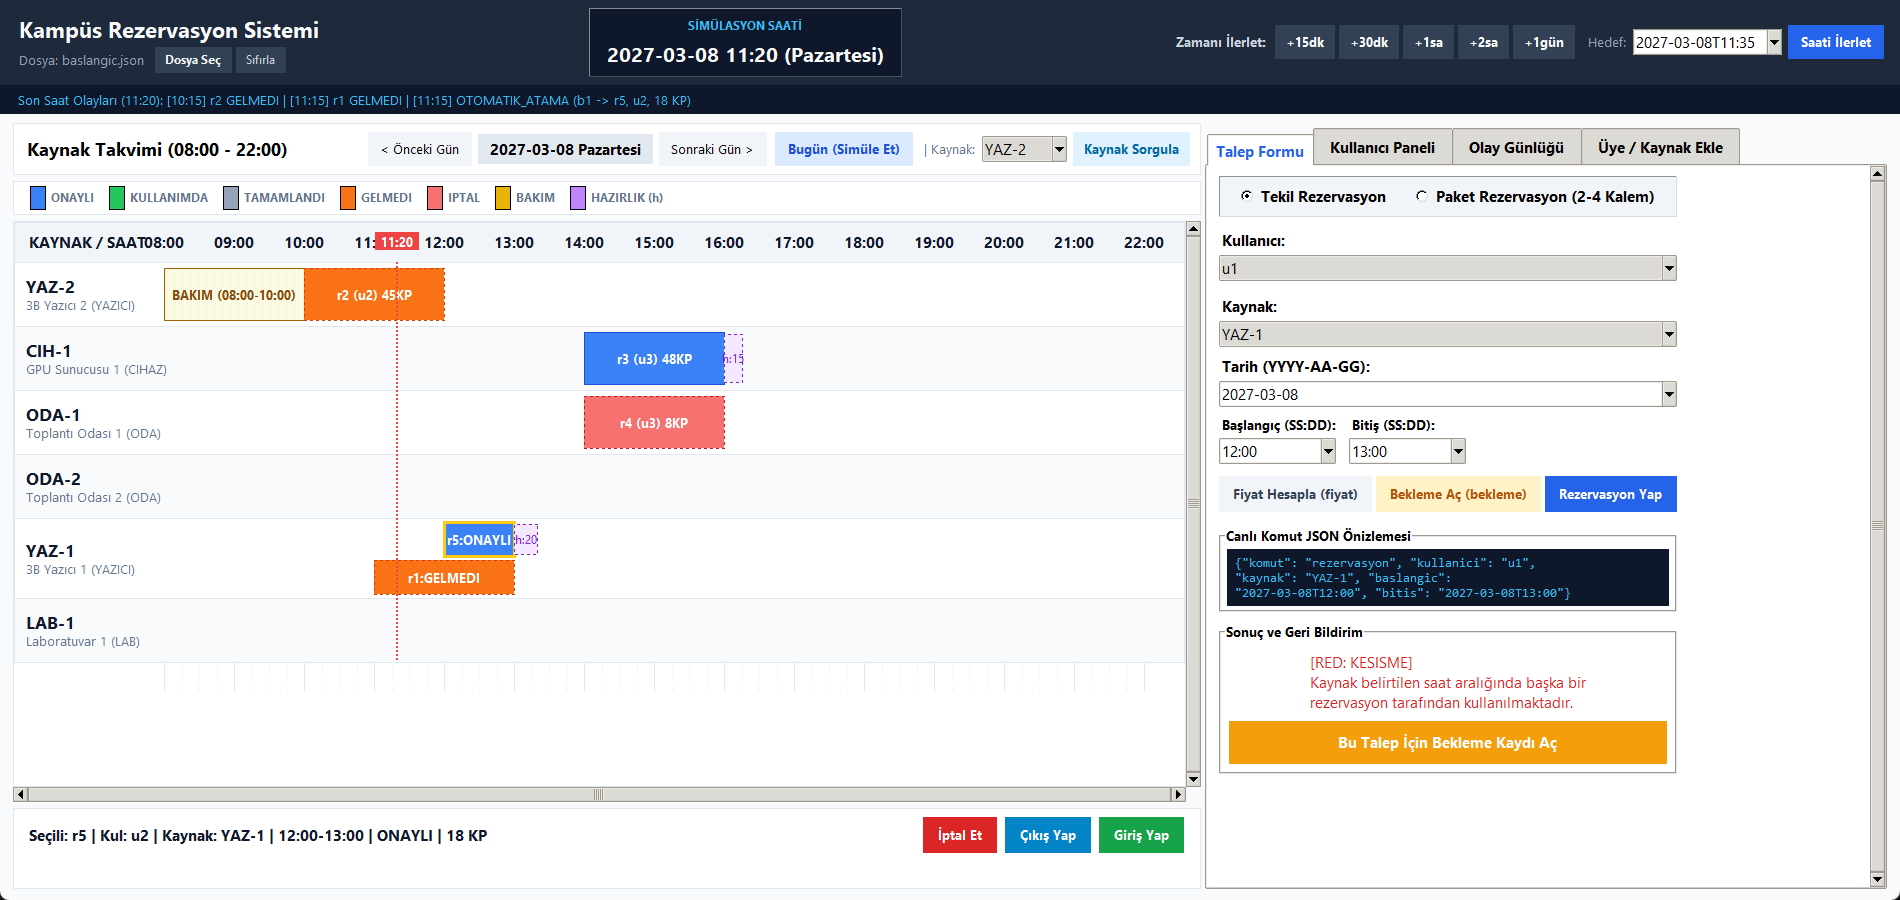
\includegraphics[width=0.92\textwidth,keepaspectratio]{arayuz_ekran.png}
\vspace{-4pt}
\caption{Masaüstü Uygulaması Genel Görünümü: Sol takvimde kaynak bazlı alt şeritler (\texttt{YAZ-1} üzerinde \texttt{r1:GELMEDI} ve otomatik atanan \texttt{r5:ONAYLI} + \texttt{h:20} hazırlık süresi), bakım penceresi ve simüle saat çizgisi; sağ panelde talep formu, canlı komut JSON önizlemesi ve tek tıkla bekleme kaydı geri bildirimi.}
\label{fig:arayuz}
\vspace{-6pt}
\end{figure*}

\section{TASARIM KARARLARI}

\subsection{Masaüstü Arayüz Ergonomisi}
Masaüstü uygulaması, şartname Bölüm 7'deki 9 bileşeni ve 5 değerlendirme ölçütünü karşılayacak biçimde tek pencere üzerinde tasarlanmıştır (Şekil~\ref{fig:arayuz}):
\begin{itemize}
    \item \textbf{Doğrudan Eylemler:} Kullanıcı paneli, talep formları ve takvim tek pencerede toplanmıştır. Seçilen rezervasyon için \texttt{giris}, \texttt{cikis} ve \texttt{iptal} işlemleri hem takvim alt çubuğundan hem de kullanıcı panelinden rezervasyon numarası yazılmadan yürütülür.
    \item \textbf{Alt Şerit (Sub-lane) Çakışma Yönetimi:} Aynı kaynakta \texttt{IPTAL} veya \texttt{GELMEDI} durumundaki bir rezervasyon ile yeni alınan bir rezervasyon (veya hazırlık süresi) çakıştığında, kutular üst üste binmez; kaynak satırı içinde ayrı alt şeritlerde birlikte çizilir.
    \item \textbf{Canlı Komut JSON Önizlemesi ve Seçilebilir Girdiler:} Tarih, başlangıç/bitiş saati, hedef saat ve bakiye/güvenilirlik alanları seçilebilir \texttt{Combobox} bileşenleriyle sunulmuştur. Tekil ve paket talep formlarında seçilen parametrelerin üreteceği JSON komutu (\texttt{rezervasyon} veya \texttt{paket}) form üzerinde canlı olarak önizlenir.
    \item \textbf{Diyalogsuz Geri Bildirim ve Hızlı Bekleme:} Onay pencereleri (\texttt{messagebox}) kullanılmamıştır. \texttt{PAKET\_RED} durumunda her kalemin sonucu kendi satırında gösterilir; \texttt{KESISME} veya \texttt{HAZIRLIK\_IHLALI} reddinde ise bilgileri yeniden girmeden tek tıkla bekleme kaydı açılabilir.
    \item \textbf{Bölüm 5 Uyumlu Olay Günlüğü:} Olay günlüğünde seçilen satırın komut karşılığı ve modül çıktısı Bölüm 5'teki JSON biçimiyle (\texttt{no}, \texttt{komut}, \texttt{durum}, \dots) gösterilir.
\end{itemize}

\subsection{İş Kuralı Yalıtımı}
Masaüstü arayüzü (\texttt{arayuz.py}) iş kuralı barındırmaz. Geçersiz talepler arayüzde engellenmez; doğrudan çekirdek modüle iletilir ve modülün döndürdüğü hata kodu Türkçe açıklamasıyla ekranda gösterilir. Böylece CLI ve GUI aynı karar mekanizmasını paylaşır.

\subsection{Standart Kütüphane Kullanımı}
Yazılımda harici paketler yerine yalnızca Python 3.11 standart kütüphaneleri (\texttt{dataclasses}, \texttt{datetime}, \texttt{json}, \texttt{math}, \texttt{tkinter}) kullanılmıştır. Bu tercih sayesinde program ek kurulum gerektirmeden \texttt{calistir.sh} veya \texttt{calistir.bat} ile doğrudan çalıştırılabilir.

\section{SONUÇ}
Bu çalışmada, Kampüs Kaynak Rezervasyon Sistemi için arayüzden bağımsız bir çekirdek modül ve Tkinter tabanlı masaüstü uygulaması geliştirilmiştir. Python 3.11 standart kütüphanesiyle yazılan sistem; 13 adımlı doğrulama sırası, 15 dakikalık dilimlerle hesaplanan dinamik ücretlendirme ve olay tabanlı simüle saat ilerletme mekanizmalarını içerir. Modül, 19 komutluk referans senaryoda ve 72 komutluk sınır değer testlerinde beklenen çıktılarla birebir eşleşmiştir.

\begin{thebibliography}{00}
\bibitem{coffman1996} E.~G.~Coffman, M.~R.~Garey, and D.~S.~Johnson, ``Approximation algorithms for bin packing: A survey,'' in \textit{Approximation Algorithms for NP-Hard Problems}, D.~Hochbaum, Ed. Boston, MA: PWS Publishing, 1996, pp. 46--93.
\bibitem{rexford2009} J.~Rexford and A.~Greenberg, ``Network virtualization: Getting additional value from shared physical infrastructure,'' \textit{IEEE Communications Magazine}, vol. 47, no. 3, pp. 18--20, Mar. 2009.
\bibitem{yazlab2026} Kocaeli Üniversitesi Bilgisayar Mühendisliği Bölümü, ``Yazılım Laboratuvarı I Proje I Şartnamesi: Kampüs Kaynak Rezervasyon Sistemi,'' Teknik Şartname, Kocaeli, Türkiye, Ekim 2026.
\bibitem{python311} Python Software Foundation, ``Python 3.11 Standard Library Documentation: Data Classes, Datetime, and Tkinter GUI Framework,'' 2026. [Çevrimiçi]. Erişim: https://docs.python.org/3/
\bibitem{gamma1994} E.~Gamma, R.~Helm, R.~Johnson, and J.~Vlissides, \textit{Design Patterns: Elements of Reusable Object-Oriented Software}. Reading, MA: Addison-Wesley, 1994.
\end{thebibliography}

\end{document}
